\documentclass[]{article}
\usepackage{lmodern}
\usepackage{amssymb,amsmath}
\usepackage{ifxetex,ifluatex}
\usepackage{fixltx2e} % provides \textsubscript
\ifnum 0\ifxetex 1\fi\ifluatex 1\fi=0 % if pdftex
  \usepackage[T1]{fontenc}
  \usepackage[utf8]{inputenc}
\else % if luatex or xelatex
  \ifxetex
    \usepackage{mathspec}
  \else
    \usepackage{fontspec}
  \fi
  \defaultfontfeatures{Ligatures=TeX,Scale=MatchLowercase}
\fi
% use upquote if available, for straight quotes in verbatim environments
\IfFileExists{upquote.sty}{\usepackage{upquote}}{}
% use microtype if available
\IfFileExists{microtype.sty}{%
\usepackage{microtype}
\UseMicrotypeSet[protrusion]{basicmath} % disable protrusion for tt fonts
}{}
\usepackage[margin=1in]{geometry}
\usepackage{hyperref}
\hypersetup{unicode=true,
            pdftitle={Chapter 5: The Normal Model},
            pdfauthor={Jesse Mu},
            pdfborder={0 0 0},
            breaklinks=true}
\urlstyle{same}  % don't use monospace font for urls
\usepackage{color}
\usepackage{fancyvrb}
\newcommand{\VerbBar}{|}
\newcommand{\VERB}{\Verb[commandchars=\\\{\}]}
\DefineVerbatimEnvironment{Highlighting}{Verbatim}{commandchars=\\\{\}}
% Add ',fontsize=\small' for more characters per line
\usepackage{framed}
\definecolor{shadecolor}{RGB}{248,248,248}
\newenvironment{Shaded}{\begin{snugshade}}{\end{snugshade}}
\newcommand{\AlertTok}[1]{\textcolor[rgb]{0.94,0.16,0.16}{#1}}
\newcommand{\AnnotationTok}[1]{\textcolor[rgb]{0.56,0.35,0.01}{\textbf{\textit{#1}}}}
\newcommand{\AttributeTok}[1]{\textcolor[rgb]{0.77,0.63,0.00}{#1}}
\newcommand{\BaseNTok}[1]{\textcolor[rgb]{0.00,0.00,0.81}{#1}}
\newcommand{\BuiltInTok}[1]{#1}
\newcommand{\CharTok}[1]{\textcolor[rgb]{0.31,0.60,0.02}{#1}}
\newcommand{\CommentTok}[1]{\textcolor[rgb]{0.56,0.35,0.01}{\textit{#1}}}
\newcommand{\CommentVarTok}[1]{\textcolor[rgb]{0.56,0.35,0.01}{\textbf{\textit{#1}}}}
\newcommand{\ConstantTok}[1]{\textcolor[rgb]{0.00,0.00,0.00}{#1}}
\newcommand{\ControlFlowTok}[1]{\textcolor[rgb]{0.13,0.29,0.53}{\textbf{#1}}}
\newcommand{\DataTypeTok}[1]{\textcolor[rgb]{0.13,0.29,0.53}{#1}}
\newcommand{\DecValTok}[1]{\textcolor[rgb]{0.00,0.00,0.81}{#1}}
\newcommand{\DocumentationTok}[1]{\textcolor[rgb]{0.56,0.35,0.01}{\textbf{\textit{#1}}}}
\newcommand{\ErrorTok}[1]{\textcolor[rgb]{0.64,0.00,0.00}{\textbf{#1}}}
\newcommand{\ExtensionTok}[1]{#1}
\newcommand{\FloatTok}[1]{\textcolor[rgb]{0.00,0.00,0.81}{#1}}
\newcommand{\FunctionTok}[1]{\textcolor[rgb]{0.00,0.00,0.00}{#1}}
\newcommand{\ImportTok}[1]{#1}
\newcommand{\InformationTok}[1]{\textcolor[rgb]{0.56,0.35,0.01}{\textbf{\textit{#1}}}}
\newcommand{\KeywordTok}[1]{\textcolor[rgb]{0.13,0.29,0.53}{\textbf{#1}}}
\newcommand{\NormalTok}[1]{#1}
\newcommand{\OperatorTok}[1]{\textcolor[rgb]{0.81,0.36,0.00}{\textbf{#1}}}
\newcommand{\OtherTok}[1]{\textcolor[rgb]{0.56,0.35,0.01}{#1}}
\newcommand{\PreprocessorTok}[1]{\textcolor[rgb]{0.56,0.35,0.01}{\textit{#1}}}
\newcommand{\RegionMarkerTok}[1]{#1}
\newcommand{\SpecialCharTok}[1]{\textcolor[rgb]{0.00,0.00,0.00}{#1}}
\newcommand{\SpecialStringTok}[1]{\textcolor[rgb]{0.31,0.60,0.02}{#1}}
\newcommand{\StringTok}[1]{\textcolor[rgb]{0.31,0.60,0.02}{#1}}
\newcommand{\VariableTok}[1]{\textcolor[rgb]{0.00,0.00,0.00}{#1}}
\newcommand{\VerbatimStringTok}[1]{\textcolor[rgb]{0.31,0.60,0.02}{#1}}
\newcommand{\WarningTok}[1]{\textcolor[rgb]{0.56,0.35,0.01}{\textbf{\textit{#1}}}}
\usepackage{longtable,booktabs}
\usepackage{graphicx,grffile}
\makeatletter
\def\maxwidth{\ifdim\Gin@nat@width>\linewidth\linewidth\else\Gin@nat@width\fi}
\def\maxheight{\ifdim\Gin@nat@height>\textheight\textheight\else\Gin@nat@height\fi}
\makeatother
% Scale images if necessary, so that they will not overflow the page
% margins by default, and it is still possible to overwrite the defaults
% using explicit options in \includegraphics[width, height, ...]{}
\setkeys{Gin}{width=\maxwidth,height=\maxheight,keepaspectratio}
\IfFileExists{parskip.sty}{%
\usepackage{parskip}
}{% else
\setlength{\parindent}{0pt}
\setlength{\parskip}{6pt plus 2pt minus 1pt}
}
\setlength{\emergencystretch}{3em}  % prevent overfull lines
\providecommand{\tightlist}{%
  \setlength{\itemsep}{0pt}\setlength{\parskip}{0pt}}
\setcounter{secnumdepth}{0}
% Redefines (sub)paragraphs to behave more like sections
\ifx\paragraph\undefined\else
\let\oldparagraph\paragraph
\renewcommand{\paragraph}[1]{\oldparagraph{#1}\mbox{}}
\fi
\ifx\subparagraph\undefined\else
\let\oldsubparagraph\subparagraph
\renewcommand{\subparagraph}[1]{\oldsubparagraph{#1}\mbox{}}
\fi

%%% Use protect on footnotes to avoid problems with footnotes in titles
\let\rmarkdownfootnote\footnote%
\def\footnote{\protect\rmarkdownfootnote}

%%% Change title format to be more compact
\usepackage{titling}

% Create subtitle command for use in maketitle
\providecommand{\subtitle}[1]{
  \posttitle{
    \begin{center}\large#1\end{center}
    }
}

\setlength{\droptitle}{-2em}

  \title{Chapter 5: The Normal Model}
    \pretitle{\vspace{\droptitle}\centering\huge}
  \posttitle{\par}
    \author{Jesse Mu}
    \preauthor{\centering\large\emph}
  \postauthor{\par}
      \predate{\centering\large\emph}
  \postdate{\par}
    \date{October 7, 2016}


\begin{document}
\maketitle

{
\setcounter{tocdepth}{2}
\tableofcontents
}
\hypertarget{the-normal-model}{%
\section{The normal model}\label{the-normal-model}}

A normal variable \(Y\) with mean \(\theta\) and variance \(\sigma^2\)
(and thus standard deviation \(\sigma\)) we denote

\[Y \sim \mathcal{N}(\theta, \sigma^2)\]

and \(Y\) has PDF

\[
p(y) = \frac{1}{\sqrt{2\pi\sigma}} \text{exp}\left(-\frac{1}{2} \frac{(y - \theta)^2}{\sigma^2}\right)
\]

Due to the central limit theorem, the normal model is used all the time
to model sample averages or values known to be the additive result of
several random variables.

\begin{itemize}
\tightlist
\item
  It's useful to remember the percentage of values lying within 1, 2, or
  3 standard deviations of the mean when constructing priors: 68, 95,
  and 99.7\%, respectively.
\end{itemize}

\hypertarget{inference-for-the-mean-conditional-on-the-variance}{%
\section{Inference for the mean, conditional on the
variance}\label{inference-for-the-mean-conditional-on-the-variance}}

There are two parameters in the normal model. For simplicity, let's
first assume that the variance is known. Later we will show how we can
perform inference jointly for the mean and variance, but this result
will still be useful especially in Chapter 6, where Gibbs sampling
requires full conditional distributions of individual parameters.

To do inference assuming \(\sigma^2\) is known, we need to identify the
sampling distribution and prior distribution, since we must calculate

\begin{align}
p(\theta \mid \sigma^2, y_1, \dots, y_n) \propto p(y_1, \dots, y_n \mid \theta, \sigma^2) \times p(\theta \mid \sigma^2)
\end{align}

For the sampling distribution,

\begin{align}
p(y_1, \dots, y_n \mid \theta, \sigma^2) &= \prod_{i = 1}^n p(y_i \mid \theta, \sigma^2) \\
&= \prod_{i = 1}^n \frac{1}{\sqrt{2 \pi \sigma^2}} \text{exp}\left(-\frac{1}{2} \frac{(y_i - \theta)^2}{\sigma^2} \right) \\
&\propto \text{exp}\left[ -\frac{1}{2} \sum_{i = 1}^n \frac{(y_1 - \theta)^2}{\sigma^2} \right] \\
&\propto \text{exp}\left[ -\frac{1}{2} \left( \frac{\sum y_i^2}{\sigma^2} - 2 \frac{\theta \sum y_i}{\sigma^2} + \frac{n\theta^2}{\sigma^2} \right) \right] \\
&\propto \text{exp}\left[ -\frac{1}{2} \left( \frac{\sum y_i^2}{\sigma^2} - 2 \frac{\theta \sum y_i}{\sigma^2} + \frac{n\theta^2}{\sigma^2} \right) \right] \\
&\propto \text{exp}\left[ -\frac{1}{2} \left( \frac{\sum y_i^2}{\sigma^2} - 2 \frac{\theta \sum y_i}{\sigma^2} \right) \right]
\end{align}

From this we know two things:

\begin{enumerate}
\def\labelenumi{\arabic{enumi}.}
\tightlist
\item
  \(p(\theta \mid \sigma^2, y_1, \dots, y_n) \propto p(y_1, \dots, y_n \mid \theta, \sigma^2) \times p(\theta \mid \sigma^2)\)
  depends only on \(\{\sum y_i^2, \sum y_i\}\), so that is a sufficient
  statistic, as is \(\{\bar{y}, s^2\}\) (from which
  \(\sum y_i^2, \sum y_i\) are recoverable).
\item
  For \(p(\theta \mid \sigma^2)\) to be conjugate, the posterior needs
  to have quadratic terms in the exponential function, i.e.
  \(\text{exp}(c_1 (\theta - c_2)^2)\)
\end{enumerate}

In particular, 2 is a new strategy for trying to identify the conjugate
prior family. Since the exponential terms in the sampling model and
prior distribution must be combined to produce the same class of
posterior distribution, we must pick a prior distribution
\(\propto \text{exp}(c_1, (\theta - c_2)^2)\). Conveniently, normal
distributions themselves have these terms. We can verify that the normal
family is conjugate to the normal sampling model. Let
\(\theta \mid \sigma^2 \sim \mathcal{N}(\mu_0, \tau_0^2)\)
(interpretations of the prior parameters comes later):

\begin{align}
p(\theta \mid \sigma^2, y_1, \dots, y_n) &\propto p(y_1, \dots, y_n \mid \theta, \sigma^2) \times p(\theta \mid \sigma^2) \\
&\propto \text{exp}\left( -\frac{1}{2\sigma^2} \sum_{i=1}^n (y_i - \theta)^2 \right) \times \text{exp}\left(-\frac{1}{2 \tau_0^2} (\theta - \mu_0)^2\right) \\
&= \text{exp}\left[ -\frac{1}{2} \left( \frac{1}{\tau_0^2}(\theta^2 - 2\theta\mu_0 + \mu_0^2) + \frac{1}{\sigma^2}(\sum y_i^2 - 2\theta y_i + n\theta^2) \right) \right] \\
&= \text{exp}\left[ -\frac{1}{2} \left( \left(\frac{1}{\tau_0^2} + \frac{n}{\sigma^2}\right)\theta^2 + 2\left( \frac{\mu_0}{\tau_0^2} + \frac{\sum y_i}{\sigma^2} \right)\theta \right) \right] \\
\end{align}

To simplify this, let

\begin{itemize}
\tightlist
\item
  \(a = \frac{1}{\tau_0^2} + \frac{n}{\sigma^2}\)
\item
  \(b = \frac{\mu_0}{\tau_0^2} + \frac{\sum y_i}{\sigma^2}\)
\end{itemize}

Then

\begin{align}
p(\theta \mid \sigma^2, y_1, \dots, y_n) &\propto \text{exp}\left[ -\frac{1}{2} (a\theta^2 - 2b\theta) \right] \\
&\propto \text{exp}\left[ -\frac{1}{2}(a\theta^2 - 2b\theta + b^2/a) + \frac{1}{2} b^2 / a \right] & \text{Completing the square} \\
&\propto \text{exp}\left[ -\frac{1}{2}(a\theta^2 - 2b\theta + b^2/a) \right] &\text{Throw away constants} \\
&\propto \text{exp}\left[ -\frac{1}{2}a(\theta^2 - 2b\theta / a + b^2/a^2) \right] \\
&\propto \text{exp}\left[ -\frac{1}{2}a(\theta - b/a)^2 \right] \\
&\propto \text{exp}\left[ -\frac{1}{2}\left( \frac{\theta - b/a}{1 / \sqrt{a}} \right)^2 \right] \\
&= \text{dnorm}(\theta, b/a, 1/a).
\end{align}

Let these posterior parameters be \(\mu_n\) and \(\tau_n^2\). In later
chapters we will commonly follow this naming scheme: initial guesses of
parameters are denoted \(\theta_0\), then the posterior parameters are
denoted \(\theta_n\), i.e.~the updated parameters after a sample of size
\(n\).

Specifically,

\begin{align}
\mu_n &= b/a = \frac{\frac{1}{\tau_0^2} \mu_0 + \frac{n}{\sigma^2}\bar{y}}{\frac{1}{\tau_0^2} + \frac{n}{\sigma^2}} \\
\tau_n^2 &= \frac{1}{a} = \frac{1}{\frac{1}{\tau_0^2} + \frac{n}{\sigma^2}}.
\end{align}

So
\(\theta \mid \sigma^2, y_1, \dots, y_n \sim \mathcal{N}(\mu_n, \tau_n^2)\).

\hypertarget{combining-information}{%
\subsection{Combining information}\label{combining-information}}

Notice in the posterior parameters the frequency of \emph{inverse
variances} i.e. \(\frac{1}{\tau_0^2}, \frac{n}{\sigma^2}\). This hints
at the importance of using \textbf{precision} to understand and
parameterize our normal prior and posterior distributions. Specifically,
it is much more concise to express the above parameters in terms of
variance. Specifically, if we let \(\tilde{\tau_n^2} = 1 / \tau_n^2\),
i.e.~the posterior \emph{precision}, and similar tildes for the over
variables,

\[\tilde{\tau_n^2} = \tilde{\tau_0^2} + n\tilde{\sigma^2}\]

So intuitively, our posterior precision is a combination of our prior
belief in the precision of the true population mean of the data, plus
the (assumed known) precision, where a larger sample size \(n\)
increases this precision.

Using precision, the fact that \(\mu_n\) is a weighted average of prior
and sample information becomes more clear. Notice

\begin{align}
\mu_n &= \frac{\frac{1}{\tau_0^2}}{ \frac{1}{\tau_0^2} + \frac{n}{\sigma^2} } \mu_0 + 
\frac{\frac{n}{\sigma^2}}{ \frac{1}{\tau_0^2} + \frac{n}{\sigma^2} } \bar{y} \\
&= \frac{\tilde{\tau_0^2}}{\tilde{\tau_0^2} + n\tilde{\sigma^2}} \mu_0 + \frac{n\tilde{\sigma^2}}{\tilde{\tau_0^2} + n\tilde{\sigma^2}} \bar{y}
\end{align}

So the posterior mean is a weighted average of the prior expectation of
the mean \(\mu_0\) weighted by the precision of that mean
\(\tilde{\tau_0^2}\), and the observed sample mean \(\bar{y}\) weighted
by our sample size \(n\) and the (assumed known) precision
\(\tilde{\sigma^2}\).

How do we select \(\tau_0^2\)? One intuitive way to think about it (as
we have done with one-parameter models) is by treating our prior
parameters for \(\theta\) as derived from \(\kappa_0\) prior
``observations'' from the same (or similar) population that we are
sampling from. Then \(\mu_0\) is the average of these prior
observations, and let \(\tau_0^2 = \sigma^2 / \kappa_0\) be the variance
of the \emph{mean} of these prior observations. Then the posterior mean
simplifies quite nicely to:

\begin{align}
\mu_n &= \frac{\kappa_0}{\kappa_0 + n}\mu_0 + \frac{n}{\kappa_0 + n}\bar{y} \\
&= \frac{\kappa_0}{\kappa_n}\mu_0 + \frac{n}{\kappa_n}\bar{y} & \text{Let $\kappa_n = \kappa_0 + n$} \\
\end{align}

which is just a weighted average of \(\mu_0\) and \(\bar{y}\) given the
number of prior ``observations'' \(\kappa_0\) and the sample size \(n\).
We will take advantage of this when jointly estimating the mean and
variance for the normal model. The idea is to first estimate the
variance, then assume that variance \(\sigma^2\) is known such that
\(\tau_0^2 = \sigma^2 / \kappa_0\) can be estimated.

\hypertarget{prediction}{%
\subsection{Prediction}\label{prediction}}

To obtain the posterior predictive distribution, instead of doing
complex integration, we can use a trick.

\(\tilde{Y}\) is normally distributed with mean \(\theta\) and variance
\(\sigma^2\). This is equivalent to saying

\[\tilde{Y} = \theta + \tilde{\epsilon}\]

where \(\theta \sim \mathcal{N}(\mu_n, \tau_n^2\),
\(\tilde{\epsilon} \sim \mathcal{N}(0, \sigma^2)\). So adding these
normal distributions together gives

\[\tilde{Y} \mid \sigma^2, y_1, \dots, y_n \sim \mathcal{N}(\mu_n, \tau_n^2 + \sigma^2)\]

\hypertarget{example-midge-wing-data}{%
\subsection{Example: Midge wing data}\label{example-midge-wing-data}}

The wing lengths of 9 members of a species of ``midge'' are measured. We
are interested in estimates of the mean wing length and variance. Prior
information from other populations suggests that wing lengths are
typically around 1.9mm, so our initial estimate \(\mu_0 = 1.9\). One way
of assigning a prior estimate of the variance of the mean \(\tau_0^2\)
is to pick the spread of the prior such that all of its mass is above 0,
since wing lengths can't be negative. So we select \(\tau_0\) such that
2 standard deviations from 1.9 \textgreater{} 0: \(\tau_0 = 0.95\).

Our data are:

\begin{Shaded}
\begin{Highlighting}[]
\NormalTok{y =}\StringTok{ }\KeywordTok{c}\NormalTok{(}\FloatTok{1.64}\NormalTok{, }\FloatTok{1.70}\NormalTok{, }\FloatTok{1.72}\NormalTok{, }\FloatTok{1.74}\NormalTok{, }\FloatTok{1.82}\NormalTok{, }\FloatTok{1.82}\NormalTok{, }\FloatTok{1.82}\NormalTok{, }\FloatTok{1.90}\NormalTok{, }\FloatTok{2.08}\NormalTok{)}
\KeywordTok{mean}\NormalTok{(y)}
\end{Highlighting}
\end{Shaded}

\begin{verbatim}
## [1] 1.804444
\end{verbatim}

\begin{Shaded}
\begin{Highlighting}[]
\KeywordTok{var}\NormalTok{(y)}
\end{Highlighting}
\end{Shaded}

\begin{verbatim}
## [1] 0.01687778
\end{verbatim}

Since we are assuming for now that \(\sigma^2\) is known, let's use
\(s^2 = \sigma^2\).

Now calculating \(\mu_n, \tau_n^2\) is simply done by plugging in the
relevant formulas:

\begin{align}
\mu_n &= \frac{1.11 (1.9) + \frac{9}{0.017} 1.804}{1.11 + \frac{9}{0.017}} = 1.805 \\
\tau_n^2 &= \frac{1}{1.11 + \frac{9}{0.017}} = 0.002
\end{align}

\begin{Shaded}
\begin{Highlighting}[]
\KeywordTok{qnorm}\NormalTok{(}\KeywordTok{c}\NormalTok{(}\FloatTok{0.025}\NormalTok{, }\FloatTok{0.975}\NormalTok{), }\FloatTok{1.805}\NormalTok{, }\KeywordTok{sqrt}\NormalTok{(}\FloatTok{0.002}\NormalTok{))}
\end{Highlighting}
\end{Shaded}

\begin{verbatim}
## [1] 1.717348 1.892652
\end{verbatim}

\hypertarget{joint-inference-for-the-mean-and-variance}{%
\section{Joint inference for the mean and
variance}\label{joint-inference-for-the-mean-and-variance}}

For joint inference, we wish to compute the joint probability
distribution of \((\theta, \sigma^2)\) given the data, which proceeds
much like before

\[
p(\theta, \sigma^2 \mid y_1, \dots, y_n) = \frac{p(y_1, \dots, y_n \mid \theta, \sigma^2) p(\theta, \sigma^2)}{p(y_1, \dots, y_n)}
\]

Notice that the only real difference in this two parameter case is the
joint prior \(p(\theta, \sigma^2)\), which we should select a conjugate
prior distribution for to simplify posterior calculation.

Notice that if we split up

\[p(\theta, \sigma^2) = p(\theta \mid \sigma^2) p(\sigma^2)\] then, from
the previous section, we already know that the normal distribution is a
conjugate prior for the \(p(\theta \mid \sigma^2)\):
\(\mathcal{N}(\mu_0, \tau_0^2)\). With this selection, we have

\begin{align}
p(\theta, \sigma^2) &= p(\theta \mid \sigma^2) p(\sigma^2) \\
&= \text{dnorm}(\theta, \mu_0, \tau_0) \times p(\sigma^2) \\
\end{align}

Now if we let \(\tau_0\) depend on \(\sigma^2\) as we explored in the
previous section, this simplifies calculations. If \(\tau_0\) is not
proportional to \(\sigma^2\), then there is no good closed-form solution
for a posterior distribution, which is a ``semiconjugate'' prior; see
Chapter 6 for details. Specifically, if we let
\(\tau_0^2 = \sigma^2 / \kappa_0 \implies \tau_0 = \sigma / \sqrt{\kappa_0}\),
i.e. \(\tau_0^2\) is the variance of the mean of a sample of size
\(\kappa_0\) from a population with variance \(\sigma^2\):

\begin{align}
p(\theta, \sigma^2) &= \text{dnorm}(\theta, \mu_0, \tau = \sigma / \sqrt{\kappa_0}) \times p(\sigma^2)
\end{align}

Now we need to specify \(p(\sigma^2)\). We are told that the Gamma
distribtion (with support on \((0, \infty)\)) is not conjugate for the
normal variance, but it \emph{is} conjugate for the normal
\emph{precision} \(1 / \sigma^2\). It's not mentioned how this is
determined, but it probably has something to do with the ease of
expressing posterior estimates in terms of precision in the previous
section where \(\sigma^2\) is known.

Let \(1 / \sigma^2 \sim \text{Gamma}(a, b)\). Like we have done
previously, we would like to parameterize this distribution such that we
can interpret choices of the parameters of the prior as sensibly
conveying some prior expectation about the precision in this case. If we
let

\begin{itemize}
\tightlist
\item
  \(a = \nu_0 / 2\)
\item
  \(b = a \sigma_0^2 = \frac{\nu_0}{2}\sigma^2_0\)
\end{itemize}

We will show later that we can interpret \((\sigma^2_0, \nu_0)\) as the
sample variance and sample size of a set of prior observations.

If \(1 / \sigma^2 \sim \text{Gamma}(\nu_0 / 2, \sigma^2_0 \nu_0 / 2)\),
then notice that
\(\mathbb{E}(1 / \sigma^2) \neq 1 / \mathbb{E}(\sigma^2)\) since the
inverse is not a linear function. To calculate \(\mathbb{E}(\sigma^2)\)
requires something more complicated (law of the unconscious
statistician?), or we can use the fact that
\(\sigma^2 \sim \text{Inverse-Gamma}(\nu_0/2, \sigma^2_0 \nu_0 / 2)\),
for which

\begin{itemize}
\tightlist
\item
  \(\mathbb{E}(\sigma^2) = \frac{\sigma^2_0 \nu_0 / 2}{(\nu_0 / 2) - 1}\)
\item
  \(\text{mode}(\sigma^2) = \frac{\sigma^2_0 \nu_0 / 2}{(\nu_0 / 2) + 1}\)
\item
  \(\text{Var}(\sigma^2)\) decreases as \(\nu_0\) increases.
\end{itemize}

From this you can already intuit how \(\nu_0\) is a sample size, and
\(\sigma^2_0\) is an initial guess of the sample variance where the
expectation of \(\sigma^2\) more closely approaches \(\sigma^2_0\) as
\(\nu_0\) increases.

\hypertarget{posterior-inference}{%
\subsection{Posterior inference}\label{posterior-inference}}

Now we have fully specified (1) our prior distributions:

\begin{align}
1 / \sigma^2 &\sim \text{Gamma}(\nu_0 / 2, \sigma^2_0 \nu_0 / 2) \\
\theta \mid \sigma^2 &\sim \mathcal{N}(\mu_0, \sigma^2 / \kappa_0), \\
\end{align}

and (2) our sampling model:

\[
Y_1, \dots, Y_n \mid \theta, \sigma^2 \sim \text{ i.i.d. } \mathcal{N}(\theta,
\sigma^2)
\]

Now we wish to calculate \(p(\theta, \sigma^2 \mid y_1, \dots, y_n)\)
which we can decompose to a product of marginal and conditional
probabilities, just like the prior:

\[
p(\theta, \sigma^2 \mid y_1, \dots, y_n) =  p(\theta \mid \sigma^2, y_1, \dots, y_n) p(\sigma^2 \mid y_1, \dots, y_n)
\]

This is convenient because we already know
\(p(\theta \mid \sigma^2, y_1, \dots, y_n)\) from the one-parameter
case:

\begin{align}
\theta \mid \sigma^2, y_1, \dots y_n \sim \mathcal{N}(\mu_n, \tau_n^2)
\end{align}

where

\begin{align}
\mu_n &= \frac{ \frac{1}{\tau_0^2} \mu_0 + \frac{n}{\sigma^2} \bar{y} }{ \frac{1}{\tau_0^2} + \frac{n}{\sigma^2} } \\
&= \frac{ \frac{\kappa_0}{\sigma^2} \mu_0 + \frac{n}{\sigma^2} \bar{y} }{ \frac{\kappa_0}{\sigma^2} + \frac{n}{\sigma^2} } & \text{Sub $\tau_0^2 = \sigma^2 / \kappa_0$} \\
&= \frac{ \kappa_0 \mu_0 + n \bar{y} } { \kappa_0 + n } & \text{$\sigma^2$s cancel} \\
\end{align}

and

\begin{align}
\tau_n^2 &= \frac{1}{\frac{1}{\tau_0^2} + \frac{n}{\sigma^2}} \\
&= \frac{1}{\frac{\kappa_0}{\sigma^2} + \frac{n}{\sigma^2}} & \text{Sub $\tau_0^2 = \sigma^2 / \kappa_0$} \\
&= \frac{\sigma^2}{\kappa_0 + n}.
\end{align}

If we let \(\kappa_n = \kappa_0 + n\) (remember we will interpret
\(\kappa_0\) as a prior sample size, and \(n\) as this sample size),
then we have

\begin{align}
\theta \mid \sigma^2, y_1, \dots y_n \sim \mathcal{N}(\mu_n, \sigma^2 / \kappa_n)
\end{align}

Where like before, \(\mu_n\) is a weighted average of \(\mu_0\) and
\(\bar{y}\) dependent on the ``prior'' sample size \(\kappa_0\) and the
sample size \(n\), and \(\sigma^2 / \kappa_n\) is the sampling variance
of the sample mean given known variance \(\sigma^2\) and our ``sample
size'' \(\kappa_n\).

Recall our posterior distribution decomposition:

\[
p(\theta, \sigma^2 \mid y_1, \dots, y_n) =  p(\theta \mid \sigma^2, y_1, \dots, y_n) p(\sigma^2 \mid y_1, \dots, y_n)
\]

Once we calculate the second component, the posterior distribution of
\(\sigma^2\), we will have fully specified the joint posterior
distribution.

\begin{align}
p(\sigma^2 \mid y_1, \dots, y_n) &\propto p(\sigma^2) p(y_1, \dots, y_n \mid \sigma^2) \\
&= p(\sigma^2) \int p(y_1, \dots, y_n \mid \theta, \sigma^2) p(\theta \mid \sigma^2) \; d\theta \\
&= \text{dinverse-gamma}(\sigma^2, \nu_0 / 2, \sigma_0^2 \nu_0 / 2) \times \\ &\quad \int \left[ \left( \prod_{i = 1}^{n} p(y_i \mid \theta, \sigma^2) \right) \times \text{dnorm}(\theta, \mu_0, \sigma^2 / \kappa_0)  \right] \; d\theta \\
\end{align}

This integral is left as an exercise (Exercise 5.3). The result is that

\begin{align}
\sigma^2 \mid y_1, \dots, y_n & \sim \text{Inverse-Gamma}(\nu_n / 2, \sigma_n^2 \nu_n / 2) \\
1 / \sigma^2 \mid y_1, \dots, y_n &\sim \text{Gamma}(\nu_n / 2, \sigma_n^2 \nu_n / 2)
\end{align}

where

\begin{itemize}
\tightlist
\item
  \(\nu_n = \nu_0 + n\), like \(\kappa_n\)
\item
  \(\sigma_n^2 = \frac{1}{\nu_n} \left[ \nu_0 \sigma_0^2 + (n - 1)s^2 + \frac{\kappa_0 n}{\kappa_n} (\bar{y} - \mu_0)^2 \right]\)
\end{itemize}

\(\nu_n\) is fairly intuitive, it acts as a sample size which is the
``prior sample size'' of the variance plus the sample size \(n\).
\(\sigma_n^2\) is a bit harder to understand. There are three terms
here. The first, \(\nu_0 \sigma_0^2\), can be thought of as a prior sum
of squared observations from the sample mean (\(\nu_0\) prior samples
with variance \(\sigma_0^2\)). Similarly, \((n - 1)s^2\), where
\(s^2 = \sum_{i = 1}^n (y_i - \bar{y})^2 / (n - 1)\), is literally the
sum of squared (actually observed) observations from the sample mean.
Lastly, the third term increases the posterior variance if the observed
sample mean \((\bar{y})\) is \emph{far} away from the expected prior
mean \(\mu_0\), since this would suggest higher variance. All three
``sum of squares-ish'' terms are combined, then divided by the total
number of ``observations'' \(\nu_n = n + \nu_0\), as commonly done to
estimate variance from a sample.

\hypertarget{summary-of-posterior-inference}{%
\subsection{Summary of posterior
inference}\label{summary-of-posterior-inference}}

This is a lot to handle, since there are a lot of moving parts. In sum,
for inference with the normal model, there are four prior parameters to
specify:

\begin{itemize}
\tightlist
\item
  \(\sigma_0^2\), an initial estimate for the variance;
\item
  \(\nu_0\), a ``prior sample size'' from which the initial estimate of
  the \emph{variance} is observed;
\item
  \(\mu_0\), an initial estimate for the population mean;
\item
  \(\kappa_0\), a ``prior sample size'' from which the initial estimate
  of the \emph{mean} is observed
\end{itemize}

Then we have

\begin{itemize}
\tightlist
\item
  \(1 / \sigma^2 \sim \text{Gamma}(\nu_0 / 2, \sigma^2_0 \nu_0 / 2)\)
\item
  \(\implies \mathbb{E}(\sigma^2) = \sigma^2_0 \frac{\nu_0 / 2}{\nu_0 / 2 - 1}\)
  (use expectation of inverse gamma)
\item
  \(\theta \mid \sigma^2 \sim \mathcal{N}(\mu_0, \sigma^2 / \kappa_0)\)
\item
  \(\implies \mathbb{E}(\theta) = \mu_0\)
\end{itemize}

The updated parameters are

\begin{itemize}
\tightlist
\item
  \(\nu_n = \nu_0 + n\)
\item
  \(\sigma_n^2 = \frac{1}{\nu_n} \left[ \nu_0 \sigma_0^2 + (n - 1)s^2 + \frac{\kappa_0 n}{\kappa_n} (\bar{y} - \mu_0)^2 \right]\)
\item
  \(\mu_n = \frac{\kappa_0 \mu_0 + n\bar{y}}{\kappa_n}\)
\item
  \(\kappa_n = \kappa_0 + n\)
\end{itemize}

So that the posterior is finally

\begin{itemize}
\tightlist
\item
  \(1 / \sigma^2 \mid y_1, \dots, y_n \sim \text{Gamma}(\nu_n / 2, \sigma^2_n \nu_n / 2)\)
\item
  Where
  \(\mathbb{E}(\sigma^2 \mid y_1, \dots, y_n) = \frac{\sigma^2_n \nu_n}{2 (\nu_n / 2 - 1)}\)
  (using the expectation of the inverse gamma)
\item
  \(\theta \mid \sigma^2, y_1, \dots, y_n \sim \mathcal{N}(\mu_n, \sigma^2 / \kappa_n)\)
\item
  Where
  \(\mathbb{E}(\theta \mid y_1, \dots, y_n, \sigma^2) = \mu_n = \frac{\kappa_0 \mu_0 + n \bar{y}}{\kappa_n}\)
\end{itemize}

Note how the prior sample sizes for the variance and the mean are
decoupled because they update differently. However, it's common to set
\(\nu_0 = \kappa_0\).

\hypertarget{example}{%
\subsection{Example}\label{example}}

Back to midge wing length, although this time, we are leaving our
estimate of the variance of the population free as well.

From other populations, say that we weakly believe that our prior
estimates of the population mean and variance are \(\mu_0 = 1.9\) and
\(\sigma_0^2 = 0.01\), respectively. Since this is a weak belief we will
pick \(\kappa_0 = \nu_0 = 1\). Now our prior distributions are

\begin{itemize}
\tightlist
\item
  \(1 / \sigma^2 \sim \text{Gamma}(0.5, 0.005)\)
\item
  \(\theta \mid \sigma^2 \sim \mathcal{N}(1.9, \sigma^2 / \kappa_0)\)
\end{itemize}

Recall that our data are

\begin{Shaded}
\begin{Highlighting}[]
\NormalTok{y =}\StringTok{ }\KeywordTok{c}\NormalTok{(}\FloatTok{1.64}\NormalTok{, }\FloatTok{1.70}\NormalTok{, }\FloatTok{1.72}\NormalTok{, }\FloatTok{1.74}\NormalTok{, }\FloatTok{1.82}\NormalTok{, }\FloatTok{1.82}\NormalTok{, }\FloatTok{1.82}\NormalTok{, }\FloatTok{1.90}\NormalTok{, }\FloatTok{2.08}\NormalTok{)}
\NormalTok{n =}\StringTok{ }\KeywordTok{length}\NormalTok{(y)}
\NormalTok{ybar =}\StringTok{ }\KeywordTok{mean}\NormalTok{(y)}
\NormalTok{s2 =}\StringTok{ }\KeywordTok{var}\NormalTok{(y)}
\end{Highlighting}
\end{Shaded}

Now we calculate the parameters of the posterior distributions

\begin{itemize}
\tightlist
\item
  \(\kappa_n = \kappa_0 + n = 1 + 9 = 10\)
\item
  \(\nu_n = \nu_0 + n = 1 + 9 =10\)
\item
  \(\mu_n = \frac{\kappa_0 \mu_0 + n\bar{y}}{\kappa_n} = \frac{1.9 + 9(1.804)}{10} = 1.814\)
\item
  \begin{align}
  \sigma_n^2 &= \frac{1}{\nu_n} \left[ \nu_0 \sigma_0^2 + (n - 1)s^2 + \frac{\kappa_0 n}{\kappa_n} (\bar{y} - \mu_0)^2 \right] \\
  &= \frac{1}{10} \left[ 0.01 + 8(0.168) + \frac{9}{10} (1.804 - 1.9)^2 \right] \\
  &= \frac{1}{10} \left[ 0.01 + 0.135 + 0.008 \right] \\
  &= 0.015
  \end{align}
\end{itemize}

So our joint posterior distribution is

\begin{align}
1 / \sigma^2 \mid y_1, \dots, y_n &\sim \text{Gamma}(10/2 = 5, 10(0.015 / 2) = 0.075) \\
\theta \mid \sigma^2, y_1, \dots, y_n &\sim \mathcal{N}(1.814, \sigma^2 / 10)
\end{align}

Now we can plot the posterior distribution for various values of
\(\theta\) and \(\sigma^2\).

\begin{Shaded}
\begin{Highlighting}[]
\CommentTok{# Prior}
\NormalTok{mu0 =}\StringTok{ }\FloatTok{1.9}
\NormalTok{kappa0 =}\StringTok{ }\DecValTok{1}
\NormalTok{s20 =}\StringTok{ }\FloatTok{0.01}
\NormalTok{nu0 =}\StringTok{ }\DecValTok{1}

\NormalTok{kappan =}\StringTok{ }\NormalTok{kappa0 }\OperatorTok{+}\StringTok{ }\NormalTok{n}
\NormalTok{nun =}\StringTok{ }\NormalTok{nu0 }\OperatorTok{+}\StringTok{ }\NormalTok{n}
\NormalTok{mun =}\StringTok{ }\NormalTok{(kappa0 }\OperatorTok{*}\StringTok{ }\NormalTok{mu0 }\OperatorTok{+}\StringTok{ }\NormalTok{n }\OperatorTok{*}\StringTok{ }\NormalTok{ybar) }\OperatorTok{/}\StringTok{ }\NormalTok{kappan}
\NormalTok{s2n =}\StringTok{ }\NormalTok{(}\DecValTok{1} \OperatorTok{/}\StringTok{ }\NormalTok{nun) }\OperatorTok{*}\StringTok{ }\NormalTok{(nu0 }\OperatorTok{*}\StringTok{ }\NormalTok{s20 }\OperatorTok{+}\StringTok{ }\NormalTok{(n }\OperatorTok{-}\StringTok{ }\DecValTok{1}\NormalTok{) }\OperatorTok{*}\StringTok{ }\NormalTok{s2 }\OperatorTok{+}\StringTok{ }\NormalTok{(kappa0 }\OperatorTok{*}\StringTok{ }\NormalTok{n }\OperatorTok{/}\StringTok{ }\NormalTok{kappan) }\OperatorTok{*}\StringTok{ }\NormalTok{(ybar }\OperatorTok{-}\StringTok{ }\NormalTok{mu0)}\OperatorTok{^}\DecValTok{2}\NormalTok{)}

\NormalTok{Theta =}\StringTok{ }\KeywordTok{seq}\NormalTok{(}\FloatTok{1.6}\NormalTok{, }\FloatTok{2.0}\NormalTok{, }\DataTypeTok{by =} \FloatTok{0.005}\NormalTok{)}
\NormalTok{Sigma2 =}\StringTok{ }\KeywordTok{seq}\NormalTok{(}\DecValTok{0}\NormalTok{, }\FloatTok{0.04}\NormalTok{, }\DataTypeTok{by =} \FloatTok{0.0001}\NormalTok{)}

\KeywordTok{library}\NormalTok{(invgamma)}
\NormalTok{post.func =}\StringTok{ }\ControlFlowTok{function}\NormalTok{(theta, sigma2) \{}
  \KeywordTok{dnorm}\NormalTok{(theta, mun, }\KeywordTok{sqrt}\NormalTok{(sigma2 }\OperatorTok{/}\StringTok{ }\NormalTok{kappan)) }\OperatorTok{*}\StringTok{ }\KeywordTok{dinvgamma}\NormalTok{(sigma2, nun }\OperatorTok{/}\StringTok{ }\DecValTok{2}\NormalTok{, s2n }\OperatorTok{*}\StringTok{ }\NormalTok{nun }\OperatorTok{/}\StringTok{ }\DecValTok{2}\NormalTok{)}
\NormalTok{\}}

\NormalTok{d =}\StringTok{ }\KeywordTok{outer}\NormalTok{(Theta, Sigma2, post.func)}
\KeywordTok{rownames}\NormalTok{(d) =}\StringTok{ }\NormalTok{Theta}
\KeywordTok{colnames}\NormalTok{(d) =}\StringTok{ }\NormalTok{Sigma2}

\NormalTok{df =}\StringTok{ }\KeywordTok{melt}\NormalTok{(d)}
\KeywordTok{colnames}\NormalTok{(df) =}\StringTok{ }\KeywordTok{c}\NormalTok{(}\StringTok{'theta'}\NormalTok{, }\StringTok{'sigma2'}\NormalTok{, }\StringTok{'density'}\NormalTok{)}

\KeywordTok{ggplot}\NormalTok{(df, }\KeywordTok{aes}\NormalTok{(}\DataTypeTok{x =}\NormalTok{ theta, }\DataTypeTok{y =}\NormalTok{ sigma2, }\DataTypeTok{z =}\NormalTok{ density)) }\OperatorTok{+}
\StringTok{  }\KeywordTok{geom_contour}\NormalTok{(}\KeywordTok{aes}\NormalTok{(}\DataTypeTok{color =}\NormalTok{ ..level..)) }\OperatorTok{+}
\StringTok{  }\KeywordTok{guides}\NormalTok{(}\DataTypeTok{color =} \OtherTok{FALSE}\NormalTok{)}
\end{Highlighting}
\end{Shaded}

\begin{verbatim}
## Warning: Removed 81 rows containing non-finite values (stat_contour).
\end{verbatim}

\begin{center}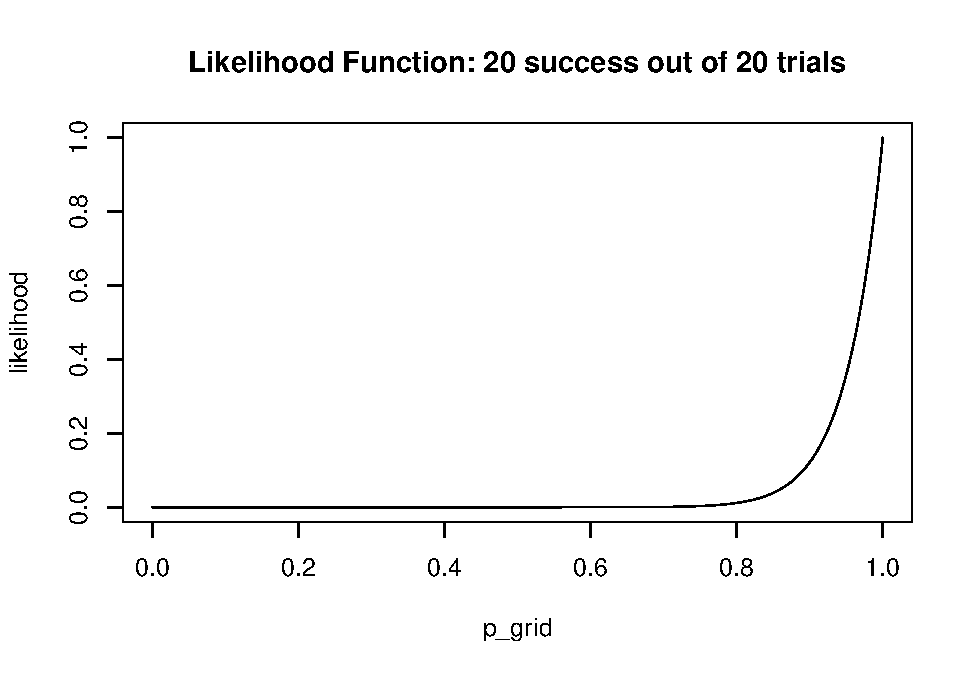
\includegraphics{5_files/figure-latex/unnamed-chunk-5-1} \end{center}

\hypertarget{monte-carlo-sampling}{%
\subsection{Monte carlo sampling}\label{monte-carlo-sampling}}

We can simulate values from the posterior by first sampling
\(\sigma^{2(n)}\) from its inverse gamma distribution, and
\(\theta^{(n)}\) from its normal distribution conditioned on
\(\sigma^{2(n)}\). Then \(\{\theta^{(n)}, \sigma^{2(n)}\}\) represent
samples from the joint distribution
\(p(\theta, \sigma^2 \mid y_1, \dots, y_n)\), and either set of values
by themselves represents samples from the full marginal distribution.
This is intuitive for \(\sigma^{2(n)}\) but less so for
\(\theta^{(n)}\). The key is to notice that, although \(\theta^{(n)}\)
is sampled conditioned on \(\sigma^{2(n)}\), multiple \(\theta^{(n)}\)
samples are conditioned on multiple \emph{different} \(\sigma^{2(n)}\)s,
so the \(\theta^{(n)}\) do indeed represent samples from the marginal
distribution.

\begin{Shaded}
\begin{Highlighting}[]
\NormalTok{s2.mc =}\StringTok{ }\KeywordTok{rinvgamma}\NormalTok{(}\DecValTok{10000}\NormalTok{, nun }\OperatorTok{/}\StringTok{ }\DecValTok{2}\NormalTok{, s2n }\OperatorTok{*}\StringTok{ }\NormalTok{nun }\OperatorTok{/}\StringTok{ }\DecValTok{2}\NormalTok{)}
\NormalTok{theta.mc =}\StringTok{ }\KeywordTok{rnorm}\NormalTok{(}\DecValTok{10000}\NormalTok{, mun, }\KeywordTok{sqrt}\NormalTok{(s2.mc }\OperatorTok{/}\StringTok{ }\NormalTok{kappan)) }\CommentTok{# Accepts a vector of parameters}
\KeywordTok{mean}\NormalTok{(theta.mc)}
\end{Highlighting}
\end{Shaded}

\begin{verbatim}
## [1] 1.813647
\end{verbatim}

\begin{Shaded}
\begin{Highlighting}[]
\KeywordTok{quantile}\NormalTok{(theta.mc, }\KeywordTok{c}\NormalTok{(}\FloatTok{0.025}\NormalTok{, }\FloatTok{0.975}\NormalTok{))}
\end{Highlighting}
\end{Shaded}

\begin{verbatim}
##     2.5%    97.5% 
## 1.727926 1.901771
\end{verbatim}

\begin{Shaded}
\begin{Highlighting}[]
\KeywordTok{ggplot}\NormalTok{(}\KeywordTok{data.frame}\NormalTok{(}\DataTypeTok{sigma2 =}\NormalTok{ s2.mc, }\DataTypeTok{theta =}\NormalTok{ theta.mc)) }\OperatorTok{+}
\StringTok{  }\KeywordTok{geom_point}\NormalTok{(}\KeywordTok{aes}\NormalTok{(}\DataTypeTok{x =}\NormalTok{ theta, }\DataTypeTok{y =}\NormalTok{ sigma2), }\DataTypeTok{alpha =} \FloatTok{0.1}\NormalTok{)}
\end{Highlighting}
\end{Shaded}

\begin{center}\includegraphics{5_files/figure-latex/unnamed-chunk-7-1} \end{center}

\hypertarget{improper-priors}{%
\subsection{Improper priors}\label{improper-priors}}

What if we want to use \emph{no} prior information? See what happens to
our posterior distribution \(\kappa_0, \nu_0 \rightarrow 0\). Using the
formula above,

\begin{itemize}
\tightlist
\item
  \(\sigma_n^2 \rightarrow \frac{n - 1}{n}s^2\)
\item
  \(\mu_n \rightarrow \bar{y}\).
\end{itemize}

Then, the ``posterior'' (plugging in \(\kappa_0 = \nu_0 = 0\) and the
posterior parameters \(\sigma_n^2, \mu_n\) and simplifying) would be

\begin{align}
1 / \sigma^2 \mid y_1, \dots, y_n &\sim \text{Gamma}(\frac{n}{2}, \frac{1}{n} \frac{n}{2}\sum (y_i - y)^2)$ \\
\theta \mid \sigma^2, y_1, \dots, y_n &\sim \mathcal{N}(\bar{y}, \frac{\sigma^2}{n})
\end{align}

With
\href{http://www.stat.columbia.edu/~fwood/Teaching/w4315/Fall2009/nuisance_parameters.pdf}{``significant
algebra''}, you can show that inference this way results in

\[\frac{\theta - \bar{y}}{s / \sqrt{n}} \mid y_1, \dots, y_n \sim t_{n - 1}\]

i.e.~a \(t\) distribution with \(n - 1\) degrees of freedom. This is
similar to the sampling distribution of \(t\) statistic:

\[\frac{\bar{Y} - \theta}{s / \sqrt{n}} \mid \theta \sim t_{n - 1}\]

but like the Bayesian vs Frequentist confidence intervals discussion in
Chapter 3, they are philosophically different. The first describes
uncertainty about the true mean conditional on the data, while the
second describes uncertainty about the observed sample mean given the
true population mean.

\hypertarget{bias-variance-and-mean-squared-error}{%
\section{Bias, variance, and mean squared
error}\label{bias-variance-and-mean-squared-error}}

Now we are diving into the properties of estimators for posterior
parameters.

\begin{quote}
A \emph{point estimator} of an unknown parameter \(\theta\) is a
function that converts your data into a single element of the parameter
space \(\Theta\). Good point estimators should hopefully approximate
(and \emph{reliably} approximate) the true value of \(\theta\); we can
formalize these properties as the bias and mean squared error of
estimators.
\end{quote}

In Bayesian analysis, point estimators are usually functions of the
posterior distribution of the parameter, such as the expectation.

The point estimator for the posterior of our normal sampling model and a
normal prior is (call it \(\hat{\theta_b}\))

\begin{align}
\hat{\theta_b} &= \frac{\kappa_0 \mu_0 + n\bar{y}}{\kappa_n} \\
&= \frac{\kappa_0}{\kappa_0 + n} \mu_0 + \frac{n}{\kappa_0 + n}\bar{y}
&= w \bar{y} + (1 - w) \mu_0
\end{align}

where \(w = \frac{n}{\kappa_0 + n}\).

\begin{quote}
The \textbf{Bias} of an estimator \(\hat{\theta}\) is
\[\text{Bias}(\hat{\theta}) = \mathbb{E}(\hat{\theta}) - \theta\]. If
\(\text{Bias}(\hat{\theta}) = 0\) we say that \(\hat{\theta}\) is an
\emph{unbiased} estimator; otherwise we say it is biased.
\end{quote}

Consider the Bayesian \(\hat{\theta_b}\) above versus the standard
maximum likelihood estimator, \(\hat{\theta_e} = \bar{y}\).

Notice that

\begin{itemize}
\tightlist
\item
  \(\text{Bias}(\hat{\theta_e}) = \mathbb{E}(\hat{\theta_e}) - \theta = 0\),
  so \(\hat{\theta_b}\) is unbiased;
\item
  \(\text{Bias}(\hat{\theta_b}) = \mathbb{E}(\hat{\theta_b}) - \theta = w\theta + (1 - w)\mu_0 - \theta\).
  Notice that the first two terms add up to \(\theta\) only if
  \(\mu_0 = \theta\). For all \(\mu \neq \theta\), \(\hat{\theta_b}\) is
  biased!
\end{itemize}

A biased estimator seems undesirable, but can actually be useful in this
setting. Imagine ``biasing'' the estimator \emph{towards the true mean}
to obtain a more accurate estimate. Thus it is useful to recall using
the Mean Squared Error as another measure of estimator performance,
which measures how close an estimator \(\hat{\theta}\) will be to the
true population parameter \(\theta\), on average:

\begin{quote}
The \textbf{Mean Squared Error} (MSE) of an estimator \(\hat{\theta}\)
is
\[\text{MSE}(\hat{\theta}) = \text{Var}(\hat{\theta}) + \text{Bias}^2(\hat{\theta})\]
\end{quote}

Let's compare the MSE of \(\hat{\theta_b}\) and \(\hat{\theta_e}\):

\begin{itemize}
\tightlist
\item
  \(\text{Var}(\hat{\theta_e}) = \text{Var}(\bar{y}) = \frac{\sigma^2}{n}\)
\item
  \(\text{Var}(\hat{\theta_b}) = \text{Var}(w \theta_0 + (1 - w)\mu_0) = \text{Var}(w \theta) = w^2 \frac{\sigma^2}{n}\)
\end{itemize}

So

\[\text{MSE}(\hat{\theta_e}) = \text{Var}(\hat{\theta_e}) + \text{Bias}^2(\hat{\theta_e}) = \frac{\sigma^2}{n} + 0\]
\begin{align}
\text{MSE}(\hat{\theta_b}) &= \text{Var}(\hat{\theta_b}) + \text{Bias}^2(\hat{\theta_b}) \\
&= w^2 \frac{\sigma^2}{n} + \left[ w\theta + (1 - w)\mu_0 - \theta \right]^2 \\
&= w^2 \frac{\sigma^2}{n} + \left[ (1 - w)\mu_0 - (1 - w)\theta \right]^2 \\
&= w^2 \frac{\sigma^2}{n} + (1 - w)^2(\mu_0 - \theta)^2 \\
\end{align}

Notice that \begin{align}
& \text{MSE}(\hat{\theta_b}) < \text{MSE}(\hat{\theta_e}) \\
\implies& w^2 \frac{\sigma^2}{n} + (1 - w)^2 (\mu_0 - \theta)^2 < \frac{\sigma^2}{n} \\
\implies& (1-w)^2(\mu_0 - \theta)^2 < (1 - w^2) \frac{\sigma^2}{n} \\
\implies& (\mu_0 - \theta)^2 < \frac{\sigma^2}{n} \frac{1-w^2}{(1 - w)^2} \\
\implies& (\mu_0 - \theta)^2 < \frac{\sigma^2}{n} \frac{(1 - w)(1 + w)}{(1 - w)^2} & \text{Difference of squares} \\
\implies& (\mu_0 - \theta)^2 < \frac{\sigma^2}{n} \frac{1 + w}{1 - w} \\
\implies& (\mu_0 - \theta)^2 < \frac{\sigma^2}{n} \frac{1 + \frac{n}{\kappa_0 + n}}{1 - \frac{n}{\kappa_0 + n}} & \text{Def. of $w$} \\
\implies& (\mu_0 - \theta)^2 < \frac{\sigma^2}{n} \frac{\frac{\kappa_0 + 2n}{\kappa_0 + n}}{\frac{\kappa_0}{\kappa_0 + n}} \\
\implies& (\mu_0 - \theta)^2 < \frac{\sigma^2}{n} \frac{\kappa_0 + 2n}{\kappa_0 + n}\frac{\kappa_0 + n}{\kappa_0} \\
\implies& (\mu_0 - \theta)^2 < \frac{\sigma^2}{n} \frac{\kappa_0 + 2n}{\kappa_0} \\
\implies& (\mu_0 - \theta)^2 < \sigma^2 \frac{\kappa_0 + 2n}{n\kappa_0} \\
\implies& (\mu_0 - \theta)^2 < \sigma^2 \left( \frac{\kappa_0}{n\kappa_0} + \frac{2n}{n\kappa_0} \right) \\
\implies& (\mu_0 - \theta)^2 < \sigma^2 \left( \frac{1}{n} + \frac{2}{\kappa_0} \right) \\
\end{align}

So the Bayesian estimator has lower mean squared error than the ML
estimate as long as values of \(\mu_0\) and \(\kappa_0\) are picked such
that this inequality holds - intutively, if your ``guess'' about the
prior is not far from the truth.

\hypertarget{prior-specification-based-on-expectations}{%
\section{Prior specification based on
expectations}\label{prior-specification-based-on-expectations}}

The normal model can be shown to be an 2-dimensional exponential model.
A \(p\)-dimensional exponential family model has densities of the form

\[p(y \mid \boldsymbol{\phi}) = h(y) c(\boldsymbol{\phi}) \text{exp}\left( \boldsymbol{\phi}^T \mathbf{t}(y) \right)\]

Recall the normal density:
\[p(y \mid \theta, \sigma^2) = \frac{1}{\sqrt{2 \pi \sigma^2}} \text{exp} \left( - \frac{(y - \theta)^2}{2\sigma^2} \right)\]
For clarity later, let's expand the quadratic term in the exponential:
\[p(y \mid \theta, \sigma^2) = \frac{1}{\sqrt{2 \pi \sigma^2}} \text{exp} \left( - \frac{y^2 - 2\theta y + \theta^2}{2\sigma^2} \right)\]

Given the exponential family parameters

\begin{itemize}
\tightlist
\item
  \(\mathbf{t}(y) = (y, y^2)\)
\item
  \(\boldsymbol{\phi} = (\theta / \sigma^2, -(2\sigma^2)^{-1})\)
\item
  \(c(\boldsymbol{\phi}) = | \phi_2 |^{1 / 2} \text{exp}\left(\phi_1^2 / (2\phi_2) \right)\)
\item
  \(h(y) = 1 / \sqrt{\pi}\)
\end{itemize}

You can reconstruct the normal density:

\begin{align}
p(y \mid \boldsymbol{\phi}) &= \frac{1}{\sqrt{\pi}} | \phi_2 |^{1/2} \text{exp}\left( \frac{\phi_1^2}{2\phi_2} \right) \text{exp} \left(\begin{pmatrix} y & y^2 \end{pmatrix}  \begin{pmatrix} \theta/\sigma^2 \\ -(2\sigma^2)^{-1} \end{pmatrix}  \right) \\
&= \frac{1}{\sqrt{\pi}} (2\sigma^2)^{-1/2} \text{exp}\left( \frac{(\theta / \sigma^2)^2}{-2(2\sigma^2)^{-1}} \right) \text{exp} \left(\begin{pmatrix} y & y^2 \end{pmatrix}  \begin{pmatrix} \theta/\sigma^2 \\ -(2\sigma^2)^{-1} \end{pmatrix} \right) \\
\end{align}

I am not going to do the exact algebra here, but notice that once you
combine the exponential terms (and the matrix multiplication in the
second exp), there are three separate terms added together. With a
common factor of \(1 / -2\sigma^2\), those three terms are the \(y^2\),
\(2 \theta y\), and \(\theta^2\) of the expanded normal density above.

With exponential family models, we can now ``read off'' conjugate
priors; for the \(p\)-dimensional case, the prior is
\(p(\boldsymbol{\phi} \mid n_0, \mathbf{t}_0) \propto c(\boldsymbol{\phi})^{n_0} \text{exp}(n_0 \mathbf{t}_0^T \boldsymbol{\phi})\).
Using the change of variables formula (which seems very complicated),
you can reparamaterize the corresponding prior in terms of \(\theta\)
and \(\sigma^2\), which gives a prior that is the product of two priors
we had determined previously to be conjugate: the normal and
inverse-gamma densities.

There are some more details on the significance of specifying \(n_0\)
and \(\mathbf{t}_0\) that I am skipping, since it essentially mirrors
the prior specification advice in the previous sections.

\hypertarget{normal-model-for-non-normal-data}{%
\section{Normal model for non-normal
data}\label{normal-model-for-non-normal-data}}

Because of the central limit theorem etc., we often use the normal model
for non-normal data. This is especially applicable when 1) we are
measuring summary statistics of a population, such as the mean, and 2)
when we are measuring variables that might be the additive result of
many underlying factors, which results in an approximately normal
variable.

\hypertarget{exercises}{%
\section{Exercises}\label{exercises}}

\hypertarget{section}{%
\subsection{5.1}\label{section}}

\begin{Shaded}
\begin{Highlighting}[]
\NormalTok{school1 =}\StringTok{ }\KeywordTok{scan}\NormalTok{(}\StringTok{'http://www.stat.washington.edu/people/pdhoff/Book/Data/hwdata/school1.dat'}\NormalTok{)}
\NormalTok{school2 =}\StringTok{ }\KeywordTok{scan}\NormalTok{(}\StringTok{'http://www.stat.washington.edu/people/pdhoff/Book/Data/hwdata/school2.dat'}\NormalTok{)}
\NormalTok{school3 =}\StringTok{ }\KeywordTok{scan}\NormalTok{(}\StringTok{'http://www.stat.washington.edu/people/pdhoff/Book/Data/hwdata/school3.dat'}\NormalTok{)}
\end{Highlighting}
\end{Shaded}

\hypertarget{a}{%
\subsubsection{a}\label{a}}

\begin{Shaded}
\begin{Highlighting}[]
\NormalTok{mu0 =}\StringTok{ }\DecValTok{5}
\NormalTok{s20 =}\StringTok{ }\DecValTok{4}
\NormalTok{k0 =}\StringTok{ }\DecValTok{1}
\NormalTok{nu0 =}\StringTok{ }\DecValTok{2}

\NormalTok{params =}\StringTok{ }\KeywordTok{lapply}\NormalTok{(}\KeywordTok{list}\NormalTok{(school1, school2, school3), }\ControlFlowTok{function}\NormalTok{(sdata) \{}
  \CommentTok{# Statistics of data}
\NormalTok{  n =}\StringTok{ }\KeywordTok{length}\NormalTok{(sdata)}
\NormalTok{  ybar =}\StringTok{ }\KeywordTok{mean}\NormalTok{(sdata)}
\NormalTok{  s2 =}\StringTok{ }\KeywordTok{var}\NormalTok{(sdata)}
  
  \CommentTok{# Compute posterior values, mun, s2n, kappan, nun}
\NormalTok{  kn =}\StringTok{ }\NormalTok{k0 }\OperatorTok{+}\StringTok{ }\NormalTok{n}
\NormalTok{  nun =}\StringTok{ }\NormalTok{nu0 }\OperatorTok{+}\StringTok{ }\NormalTok{n}
\NormalTok{  mun =}\StringTok{ }\NormalTok{(k0 }\OperatorTok{*}\StringTok{ }\NormalTok{mu0 }\OperatorTok{+}\StringTok{ }\NormalTok{n }\OperatorTok{*}\StringTok{ }\NormalTok{ybar) }\OperatorTok{/}\StringTok{ }\NormalTok{kn}
\NormalTok{  s2n =}\StringTok{ }\NormalTok{(}\DecValTok{1} \OperatorTok{/}\StringTok{ }\NormalTok{nun) }\OperatorTok{*}\StringTok{ }\NormalTok{(nu0 }\OperatorTok{*}\StringTok{ }\NormalTok{s20 }\OperatorTok{+}\StringTok{ }\NormalTok{(n }\OperatorTok{-}\StringTok{ }\DecValTok{1}\NormalTok{) }\OperatorTok{*}\StringTok{ }\NormalTok{s2 }\OperatorTok{+}\StringTok{ }\NormalTok{((k0 }\OperatorTok{*}\StringTok{ }\NormalTok{n) }\OperatorTok{/}\StringTok{ }\NormalTok{kn) }\OperatorTok{*}\StringTok{ }\NormalTok{(ybar }\OperatorTok{-}\StringTok{ }\NormalTok{mu0)}\OperatorTok{^}\DecValTok{2}\NormalTok{)}
  
  \KeywordTok{c}\NormalTok{(}\StringTok{'mun'}\NormalTok{ =}\StringTok{ }\NormalTok{mun, }\StringTok{'s2n'}\NormalTok{ =}\StringTok{ }\NormalTok{s2n, }\StringTok{'kn'}\NormalTok{ =}\StringTok{ }\NormalTok{kn, }\StringTok{'nun'}\NormalTok{ =}\StringTok{ }\NormalTok{nun)}
\NormalTok{\})}

\NormalTok{params.df =}\StringTok{ }\KeywordTok{as.data.frame}\NormalTok{(}\KeywordTok{rbind}\NormalTok{(params[[}\DecValTok{1}\NormalTok{]], params[[}\DecValTok{2}\NormalTok{]], params[[}\DecValTok{3}\NormalTok{]]))}
\KeywordTok{rownames}\NormalTok{(params.df) =}\StringTok{ }\KeywordTok{c}\NormalTok{(}\StringTok{'school1'}\NormalTok{, }\StringTok{'school2'}\NormalTok{, }\StringTok{'school3'}\NormalTok{)}
\end{Highlighting}
\end{Shaded}

\begin{Shaded}
\begin{Highlighting}[]
\CommentTok{# 5000 monte carlo samples. Need to estimate \textbackslash{}sigma^2 before \textbackslash{}theta.}
\CommentTok{# I can easily do means and confidence intervals of the \textbackslash{}sigma^2, but for}
\CommentTok{# brevity, I will output only \textbackslash{}theta}
\NormalTok{school1.s2.mc =}\StringTok{ }\DecValTok{1} \OperatorTok{/}\StringTok{ }\KeywordTok{rgamma}\NormalTok{(}\DecValTok{5000}\NormalTok{, params.df[}\DecValTok{1}\NormalTok{, ]}\OperatorTok{$}\NormalTok{nun }\OperatorTok{/}\StringTok{ }\DecValTok{2}\NormalTok{, params.df[}\DecValTok{1}\NormalTok{, ]}\OperatorTok{$}\NormalTok{s2n }\OperatorTok{*}\StringTok{ }\NormalTok{params.df[}\DecValTok{1}\NormalTok{, ]}\OperatorTok{$}\NormalTok{nun }\OperatorTok{/}\StringTok{ }\DecValTok{2}\NormalTok{)}
\NormalTok{school1.theta.mc =}\StringTok{ }\KeywordTok{rnorm}\NormalTok{(}\DecValTok{5000}\NormalTok{, params.df[}\DecValTok{1}\NormalTok{, ]}\OperatorTok{$}\NormalTok{mun, }\KeywordTok{sqrt}\NormalTok{(school1.s2.mc }\OperatorTok{/}\StringTok{ }\NormalTok{params.df[}\DecValTok{1}\NormalTok{, ]}\OperatorTok{$}\NormalTok{kn))}
\KeywordTok{quantile}\NormalTok{(school1.theta.mc, }\DataTypeTok{probs =} \KeywordTok{c}\NormalTok{(}\FloatTok{0.025}\NormalTok{, }\FloatTok{0.5}\NormalTok{, }\FloatTok{0.975}\NormalTok{))}
\end{Highlighting}
\end{Shaded}

\begin{verbatim}
##      2.5%       50%     97.5% 
##  7.786852  9.283342 10.862010
\end{verbatim}

\begin{Shaded}
\begin{Highlighting}[]
\NormalTok{school2.s2.mc =}\StringTok{ }\DecValTok{1} \OperatorTok{/}\StringTok{ }\KeywordTok{rgamma}\NormalTok{(}\DecValTok{5000}\NormalTok{, params.df[}\DecValTok{2}\NormalTok{, ]}\OperatorTok{$}\NormalTok{nun }\OperatorTok{/}\StringTok{ }\DecValTok{2}\NormalTok{, params.df[}\DecValTok{2}\NormalTok{, ]}\OperatorTok{$}\NormalTok{s2n }\OperatorTok{*}\StringTok{ }\NormalTok{params.df[}\DecValTok{2}\NormalTok{, ]}\OperatorTok{$}\NormalTok{nun }\OperatorTok{/}\StringTok{ }\DecValTok{2}\NormalTok{)}
\NormalTok{school2.theta.mc =}\StringTok{ }\KeywordTok{rnorm}\NormalTok{(}\DecValTok{5000}\NormalTok{, params.df[}\DecValTok{2}\NormalTok{, ]}\OperatorTok{$}\NormalTok{mun, }\KeywordTok{sqrt}\NormalTok{(school2.s2.mc }\OperatorTok{/}\StringTok{ }\NormalTok{params.df[}\DecValTok{2}\NormalTok{, ]}\OperatorTok{$}\NormalTok{kn))}
\KeywordTok{quantile}\NormalTok{(school2.theta.mc, }\DataTypeTok{probs =} \KeywordTok{c}\NormalTok{(}\FloatTok{0.025}\NormalTok{, }\FloatTok{0.5}\NormalTok{, }\FloatTok{0.975}\NormalTok{))}
\end{Highlighting}
\end{Shaded}

\begin{verbatim}
##     2.5%      50%    97.5% 
## 5.122142 6.928974 8.692013
\end{verbatim}

\begin{Shaded}
\begin{Highlighting}[]
\NormalTok{school3.s2.mc =}\StringTok{ }\DecValTok{1} \OperatorTok{/}\StringTok{ }\KeywordTok{rgamma}\NormalTok{(}\DecValTok{5000}\NormalTok{, params.df[}\DecValTok{3}\NormalTok{, ]}\OperatorTok{$}\NormalTok{nun }\OperatorTok{/}\StringTok{ }\DecValTok{3}\NormalTok{, params.df[}\DecValTok{3}\NormalTok{, ]}\OperatorTok{$}\NormalTok{s2n }\OperatorTok{*}\StringTok{ }\NormalTok{params.df[}\DecValTok{3}\NormalTok{, ]}\OperatorTok{$}\NormalTok{nun }\OperatorTok{/}\StringTok{ }\DecValTok{2}\NormalTok{)}
\NormalTok{school3.theta.mc =}\StringTok{ }\KeywordTok{rnorm}\NormalTok{(}\DecValTok{5000}\NormalTok{, params.df[}\DecValTok{3}\NormalTok{, ]}\OperatorTok{$}\NormalTok{mun, }\KeywordTok{sqrt}\NormalTok{(school3.s2.mc }\OperatorTok{/}\StringTok{ }\NormalTok{params.df[}\DecValTok{3}\NormalTok{, ]}\OperatorTok{$}\NormalTok{kn))}
\KeywordTok{quantile}\NormalTok{(school3.theta.mc, }\DataTypeTok{probs =} \KeywordTok{c}\NormalTok{(}\FloatTok{0.025}\NormalTok{, }\FloatTok{0.5}\NormalTok{, }\FloatTok{0.975}\NormalTok{))}
\end{Highlighting}
\end{Shaded}

\begin{verbatim}
##     2.5%      50%    97.5% 
## 5.696942 7.797351 9.893959
\end{verbatim}

\hypertarget{b}{%
\subsubsection{b}\label{b}}

\begin{Shaded}
\begin{Highlighting}[]
\KeywordTok{library}\NormalTok{(combinat)}
\NormalTok{school.theta.mc =}\StringTok{ }\KeywordTok{list}\NormalTok{(school1.theta.mc, school2.theta.mc, school3.theta.mc)}
\NormalTok{perms =}\StringTok{ }\KeywordTok{permn}\NormalTok{(}\DecValTok{1}\OperatorTok{:}\DecValTok{3}\NormalTok{)}
\NormalTok{theta.lt.probs =}\StringTok{ }\KeywordTok{lapply}\NormalTok{(perms, }\ControlFlowTok{function}\NormalTok{(perm) \{}
  \CommentTok{# This is a vector e.g. c(1, 3, 2)}
  \KeywordTok{mean}\NormalTok{(school.theta.mc[[perm[}\DecValTok{1}\NormalTok{]]] }\OperatorTok{<}\StringTok{ }\NormalTok{school.theta.mc[[perm[}\DecValTok{2}\NormalTok{]]] }\OperatorTok{&}
\StringTok{         }\NormalTok{school.theta.mc[[perm[}\DecValTok{2}\NormalTok{]]] }\OperatorTok{<}\StringTok{ }\NormalTok{school.theta.mc[[perm[}\DecValTok{3}\NormalTok{]]])}
\NormalTok{\})}
\KeywordTok{names}\NormalTok{(theta.lt.probs) =}\StringTok{ }\KeywordTok{sapply}\NormalTok{(perms, }\ControlFlowTok{function}\NormalTok{(v) }\KeywordTok{paste}\NormalTok{(v, }\DataTypeTok{collapse =}\StringTok{' < '}\NormalTok{))}
\NormalTok{theta.lt.probs.stacked =}\StringTok{ }\KeywordTok{stack}\NormalTok{(theta.lt.probs)[, }\KeywordTok{c}\NormalTok{(}\DecValTok{2}\NormalTok{, }\DecValTok{1}\NormalTok{)] }\CommentTok{# Reverse stack order}
\KeywordTok{kable}\NormalTok{(theta.lt.probs.stacked, }\DataTypeTok{col.names =} \KeywordTok{c}\NormalTok{(}\StringTok{'inequality'}\NormalTok{, }\StringTok{'prob'}\NormalTok{))}
\end{Highlighting}
\end{Shaded}

\begin{longtable}[]{@{}lr@{}}
\toprule
inequality & prob\tabularnewline
\midrule
\endhead
1 \textless{} 2 \textless{} 3 & 0.0070\tabularnewline
1 \textless{} 3 \textless{} 2 & 0.0026\tabularnewline
3 \textless{} 1 \textless{} 2 & 0.0130\tabularnewline
3 \textless{} 2 \textless{} 1 & 0.2478\tabularnewline
2 \textless{} 3 \textless{} 1 & 0.6172\tabularnewline
2 \textless{} 1 \textless{} 3 & 0.1124\tabularnewline
\bottomrule
\end{longtable}

\hypertarget{c}{%
\subsubsection{c}\label{c}}

\begin{Shaded}
\begin{Highlighting}[]
\NormalTok{school.s2.mc =}\StringTok{ }\KeywordTok{list}\NormalTok{(school1.s2.mc, school2.s2.mc, school3.s2.mc)}
\NormalTok{school.y.mc =}\StringTok{ }\KeywordTok{lapply}\NormalTok{(}\DecValTok{1}\OperatorTok{:}\DecValTok{3}\NormalTok{, }\ControlFlowTok{function}\NormalTok{(i) \{}
\NormalTok{  this.s2 =}\StringTok{ }\NormalTok{school.s2.mc[[i]]}
\NormalTok{  this.theta =}\StringTok{ }\NormalTok{school.theta.mc[[i]]}
  \KeywordTok{rnorm}\NormalTok{(}\DecValTok{5000}\NormalTok{, this.theta, }\KeywordTok{sqrt}\NormalTok{(this.s2))}
\NormalTok{\})}
\NormalTok{y.lt.probs =}\StringTok{ }\KeywordTok{lapply}\NormalTok{(perms, }\ControlFlowTok{function}\NormalTok{(perm) \{}
  \CommentTok{# This is a vector e.g. c(1, 3, 2)}
  \KeywordTok{mean}\NormalTok{(school.y.mc[[perm[}\DecValTok{1}\NormalTok{]]] }\OperatorTok{<}\StringTok{ }\NormalTok{school.y.mc[[perm[}\DecValTok{2}\NormalTok{]]] }\OperatorTok{&}
\StringTok{         }\NormalTok{school.y.mc[[perm[}\DecValTok{2}\NormalTok{]]] }\OperatorTok{<}\StringTok{ }\NormalTok{school.y.mc[[perm[}\DecValTok{3}\NormalTok{]]])}
\NormalTok{\})}
\KeywordTok{names}\NormalTok{(y.lt.probs) =}\StringTok{ }\KeywordTok{sapply}\NormalTok{(perms, }\ControlFlowTok{function}\NormalTok{(v) }\KeywordTok{paste}\NormalTok{(v, }\DataTypeTok{collapse =}\StringTok{' < '}\NormalTok{))}
\NormalTok{y.lt.probs.stacked =}\StringTok{ }\KeywordTok{stack}\NormalTok{(y.lt.probs)[, }\KeywordTok{c}\NormalTok{(}\DecValTok{2}\NormalTok{, }\DecValTok{1}\NormalTok{)] }\CommentTok{# Reverse stack order}
\KeywordTok{kable}\NormalTok{(y.lt.probs.stacked, }\DataTypeTok{col.names =} \KeywordTok{c}\NormalTok{(}\StringTok{'inequality'}\NormalTok{, }\StringTok{'prob'}\NormalTok{))}
\end{Highlighting}
\end{Shaded}

\begin{longtable}[]{@{}lr@{}}
\toprule
inequality & prob\tabularnewline
\midrule
\endhead
1 \textless{} 2 \textless{} 3 & 0.1154\tabularnewline
1 \textless{} 3 \textless{} 2 & 0.0918\tabularnewline
3 \textless{} 1 \textless{} 2 & 0.1378\tabularnewline
3 \textless{} 2 \textless{} 1 & 0.2194\tabularnewline
2 \textless{} 3 \textless{} 1 & 0.2376\tabularnewline
2 \textless{} 1 \textless{} 3 & 0.1980\tabularnewline
\bottomrule
\end{longtable}

\hypertarget{d}{%
\subsubsection{d}\label{d}}

\begin{Shaded}
\begin{Highlighting}[]
\NormalTok{theta1.big.prob =}\StringTok{ }\KeywordTok{mean}\NormalTok{(school.theta.mc[[}\DecValTok{1}\NormalTok{]] }\OperatorTok{>}\StringTok{ }\NormalTok{school.theta.mc[[}\DecValTok{2}\NormalTok{]] }\OperatorTok{&}\StringTok{ }\NormalTok{school.theta.mc[[}\DecValTok{1}\NormalTok{]] }\OperatorTok{>}\StringTok{ }\NormalTok{school.theta.mc[[}\DecValTok{3}\NormalTok{]])}
\KeywordTok{print}\NormalTok{(theta1.big.prob)}
\end{Highlighting}
\end{Shaded}

\begin{verbatim}
## [1] 0.865
\end{verbatim}

\begin{Shaded}
\begin{Highlighting}[]
\NormalTok{y1.big.prob =}\StringTok{ }\KeywordTok{mean}\NormalTok{(school.y.mc[[}\DecValTok{1}\NormalTok{]] }\OperatorTok{>}\StringTok{ }\NormalTok{school.y.mc[[}\DecValTok{2}\NormalTok{]] }\OperatorTok{&}\StringTok{ }\NormalTok{school.y.mc[[}\DecValTok{1}\NormalTok{]] }\OperatorTok{>}\StringTok{ }\NormalTok{school.y.mc[[}\DecValTok{3}\NormalTok{]])}
\KeywordTok{print}\NormalTok{(y1.big.prob)}
\end{Highlighting}
\end{Shaded}

\begin{verbatim}
## [1] 0.457
\end{verbatim}

\hypertarget{section-1}{%
\subsection{5.2}\label{section-1}}

\begin{Shaded}
\begin{Highlighting}[]
\NormalTok{mu0 =}\StringTok{ }\DecValTok{75}
\NormalTok{s20 =}\StringTok{ }\DecValTok{100}

\NormalTok{n.a =}\StringTok{ }\NormalTok{n.b =}\StringTok{ }\DecValTok{16}
\NormalTok{ybar.a =}\StringTok{ }\FloatTok{75.2}
\NormalTok{s2.a =}\StringTok{ }\FloatTok{7.3}\OperatorTok{^}\DecValTok{2}
\NormalTok{ybar.b =}\StringTok{ }\FloatTok{77.5}
\NormalTok{s2.b =}\StringTok{ }\FloatTok{8.1}\OperatorTok{^}\DecValTok{2}

\NormalTok{k0nu0 =}\StringTok{ }\KeywordTok{c}\NormalTok{(}\DecValTok{1}\NormalTok{, }\DecValTok{2}\NormalTok{, }\DecValTok{4}\NormalTok{, }\DecValTok{8}\NormalTok{, }\DecValTok{16}\NormalTok{, }\DecValTok{32}\NormalTok{)}

\NormalTok{prob =}\StringTok{ }\KeywordTok{sapply}\NormalTok{(k0nu0, }\ControlFlowTok{function}\NormalTok{(p) \{}
  \CommentTok{# p is the common parameter for k0 and nu0}
  
  \CommentTok{# Calculate posterior parameters}
\NormalTok{  kn.a =}\StringTok{ }\NormalTok{p }\OperatorTok{+}\StringTok{ }\NormalTok{n.a}
\NormalTok{  nun.a =}\StringTok{ }\NormalTok{p }\OperatorTok{+}\StringTok{ }\NormalTok{n.a}
\NormalTok{  mun.a =}\StringTok{ }\NormalTok{(p }\OperatorTok{*}\StringTok{ }\NormalTok{mu0 }\OperatorTok{+}\StringTok{ }\NormalTok{n.a }\OperatorTok{*}\StringTok{ }\NormalTok{ybar.a) }\OperatorTok{/}\StringTok{ }\NormalTok{kn.a}
\NormalTok{  s2n.a =}\StringTok{ }\NormalTok{(}\DecValTok{1} \OperatorTok{/}\StringTok{ }\NormalTok{nun.a) }\OperatorTok{*}\StringTok{ }\NormalTok{(p }\OperatorTok{*}\StringTok{ }\NormalTok{s20 }\OperatorTok{+}\StringTok{ }\NormalTok{(n.a }\OperatorTok{-}\StringTok{ }\DecValTok{1}\NormalTok{) }\OperatorTok{*}\StringTok{ }\NormalTok{s2.a }\OperatorTok{+}\StringTok{ }\NormalTok{((p }\OperatorTok{*}\StringTok{ }\NormalTok{n.a) }\OperatorTok{/}\StringTok{ }\NormalTok{kn.a) }\OperatorTok{*}\StringTok{ }\NormalTok{(ybar.a }\OperatorTok{-}\StringTok{ }\NormalTok{mu0)}\OperatorTok{^}\DecValTok{2}\NormalTok{)}
  
\NormalTok{  s2.a.mc =}\StringTok{ }\DecValTok{1} \OperatorTok{/}\StringTok{ }\KeywordTok{rgamma}\NormalTok{(}\DecValTok{10000}\NormalTok{, nun.a }\OperatorTok{/}\StringTok{ }\DecValTok{2}\NormalTok{, s2n.a }\OperatorTok{*}\StringTok{ }\NormalTok{nun.a }\OperatorTok{/}\StringTok{ }\DecValTok{2}\NormalTok{)}
\NormalTok{  theta.a.mc =}\StringTok{ }\KeywordTok{rnorm}\NormalTok{(}\DecValTok{10000}\NormalTok{, mun.a, }\KeywordTok{sqrt}\NormalTok{(s2.a.mc))}
  
\NormalTok{  kn.b =}\StringTok{ }\NormalTok{p }\OperatorTok{+}\StringTok{ }\NormalTok{n.b}
\NormalTok{  nun.b =}\StringTok{ }\NormalTok{p }\OperatorTok{+}\StringTok{ }\NormalTok{n.b}
\NormalTok{  mun.b =}\StringTok{ }\NormalTok{(p }\OperatorTok{*}\StringTok{ }\NormalTok{mu0 }\OperatorTok{+}\StringTok{ }\NormalTok{n.b }\OperatorTok{*}\StringTok{ }\NormalTok{ybar.b) }\OperatorTok{/}\StringTok{ }\NormalTok{kn.b}
\NormalTok{  s2n.b =}\StringTok{ }\NormalTok{(}\DecValTok{1} \OperatorTok{/}\StringTok{ }\NormalTok{nun.b) }\OperatorTok{*}\StringTok{ }\NormalTok{(p }\OperatorTok{*}\StringTok{ }\NormalTok{s20 }\OperatorTok{+}\StringTok{ }\NormalTok{(n.b }\OperatorTok{-}\StringTok{ }\DecValTok{1}\NormalTok{) }\OperatorTok{*}\StringTok{ }\NormalTok{s2.b }\OperatorTok{+}\StringTok{ }\NormalTok{((p }\OperatorTok{*}\StringTok{ }\NormalTok{n.b) }\OperatorTok{/}\StringTok{ }\NormalTok{kn.b) }\OperatorTok{*}\StringTok{ }\NormalTok{(ybar.b }\OperatorTok{-}\StringTok{ }\NormalTok{mu0)}\OperatorTok{^}\DecValTok{2}\NormalTok{)}
  
\NormalTok{  s2.b.mc =}\StringTok{ }\DecValTok{1} \OperatorTok{/}\StringTok{ }\KeywordTok{rgamma}\NormalTok{(}\DecValTok{10000}\NormalTok{, nun.b }\OperatorTok{/}\StringTok{ }\DecValTok{2}\NormalTok{, s2n.b }\OperatorTok{*}\StringTok{ }\NormalTok{nun.b }\OperatorTok{/}\StringTok{ }\DecValTok{2}\NormalTok{)}
\NormalTok{  theta.b.mc =}\StringTok{ }\KeywordTok{rnorm}\NormalTok{(}\DecValTok{10000}\NormalTok{, mun.b, }\KeywordTok{sqrt}\NormalTok{(s2.b.mc))}
  
  \KeywordTok{mean}\NormalTok{(theta.a.mc }\OperatorTok{<}\StringTok{ }\NormalTok{theta.b.mc)}
\NormalTok{\})}

\KeywordTok{qplot}\NormalTok{(k0nu0, prob, }\DataTypeTok{geom =} \KeywordTok{c}\NormalTok{(}\StringTok{'line'}\NormalTok{, }\StringTok{'point'}\NormalTok{))}
\end{Highlighting}
\end{Shaded}

\begin{center}\includegraphics{5_files/figure-latex/unnamed-chunk-14-1} \end{center}

In general, there is weak evidence that \(\theta_A < \theta_B\).
Depending on the strength of a person's confidence in the prior, as
quantified by a ``prior sample size'' \(\nu_0 = \kappa_0\), the
posterior probability starts at \textasciitilde{}0.58 and declines as
strength increases. However, it takes a \emph{very} strong prior belief
for the probability to dip below 0.50.

\hypertarget{section-2}{%
\subsection{5.3}\label{section-2}}

I'll derive \(p(\sigma^2 \mid y_1, \dots, y_n)\):

\begin{align}
p(\sigma^2 \mid y_1, \dots, y_n) &\propto p(\sigma^2)p(y_1, \dots, y_n \mid \sigma^2) \\
&= p(\sigma^2) \times \int p(y_1, \dots, y_n \mid \theta, \sigma^2) p(\theta \mid \sigma^2) \; d\theta \\
&= \text{dinvgamma}(\sigma^2, \nu_0 / 2, \nu_0 \sigma_0^2 / 2) \int \left[ \prod_{i=1}^n \text{dnorm}(y_i, \theta, \sigma^2) \right] \times \text{dnorm}(\theta, \mu_0, \sigma^2 / \kappa_0)\; d\theta \\
&= \text{dinvgamma}(\sigma^2, \nu_0 / 2, \nu_0 \sigma_0^2 / 2) \; \times \\ &\quad \int (2\pi
\sigma^2)^{-n/2} \text{exp}\left( -\frac{1}{2} \sum \frac{(y_i -
\theta)^2}{\sigma^2} \right) \times \frac{1}{\sqrt{2\pi\sigma^2 / \kappa_0}}
\text{exp}\left(-\frac{1}{2} \frac{(\theta - \mu_0)^2}{\sigma^2 / \kappa_0}\right) \; d\theta \\
&\propto \text{dinvgamma}(\sigma^2, \nu_0 / 2, \nu_0 \sigma_0^2 / 2) \; \times \\ &\quad \sigma^{2(-(n + 1)/2)} \int \text{exp}\left( -\frac{1}{2} \sum \frac{(y_i -
\theta)^2}{\sigma^2} \right) \times 
\text{exp}\left(-\frac{1}{2} \frac{(\theta - \mu_0)^2}{\sigma^2 / \kappa_0}\right) \; d\theta \\
&\propto \dots
\end{align}

This is apparently non-trivial, and requires expanding the quadratic
terms in the \(\text{exp}\) terms. I'll skip this for now.

\hypertarget{section-3}{%
\subsection{5.4}\label{section-3}}

\hypertarget{a-1}{%
\subsubsection{a}\label{a-1}}

The log-likelihood function \(\ell\) is

\begin{align}
\ell(Y \mid \theta, \sigma^2) &= \log \left[ \frac{1}{\sqrt{2\pi\sigma^2}} \text{exp}\left(-\frac{1}{2}\sum_{i=1}^n \frac{(y_i - \theta)^2}{\sigma^2} \right) \right] \\
&= -\frac{n}{2} \log(2\pi) - \frac{n}{2}\log(\sigma^2) - \frac{1}{2\sigma^2} \sum_{i=1}^n (y_i - \theta)^2 \\
&= -\frac{n}{2} \log(2\pi) - \frac{n}{2}\log(\sigma^2) - \frac{1}{2\sigma^2} \sum_{i=1}^n y_i^2 -2\theta y_i + \theta^2 \\
&= -\frac{n}{2} \log(2\pi) - \frac{n}{2}\log(\sigma^2) - \frac{1}{2\sigma^2} \left(  \sum y_i^2 - 2\theta \sum y_i + n \theta^2 \right)
\end{align}

The first derivatives are

\begin{align}
\ell_\theta(Y \mid \theta, \sigma) &= \frac{\sum y_i - n\theta}{\sigma^2} \\
\ell_{\sigma^2}(Y \mid \theta, \sigma) &= -\frac{n}{2\sigma^2} + \frac{\sum y_i^2}{2(\sigma^2)^2} - \frac{2\theta \sum y_i}{2(\sigma^2)^2} + \frac{n\theta^2}{2(\sigma^2)^2} \\
\end{align}

So the \(2 \times 2\) matrix \(I(\theta, \sigma^2)\) is (expectations
wrt \(Y\))

\begin{align}
I(\theta, \sigma^2) &=
\begin{bmatrix}
-\mathbb{E}\left( \ell_{\theta\theta}(Y \mid \theta, \sigma) \right) & -\mathbb{E}\left( \ell_{\theta\sigma^2}(Y \mid \theta, \sigma) \right) \\
-\mathbb{E}\left( \ell_{\sigma^2\theta}(Y \mid \theta, \sigma) \right) & -\mathbb{E}\left( \ell_{\sigma^2\sigma^2}(Y \mid \theta, \sigma) \right)\\
\end{bmatrix} \\
&= \begin{bmatrix}
-\mathbb{E}\left( -\frac{n}{\sigma^2} \right) &
-\mathbb{E}\left( -\frac{\sum y_i - n\theta}{(\sigma^2)^2}\right) \\
-\mathbb{E}\left( -\frac{\sum y_i - n\theta}{(\sigma^2)^2}\right) &
-\mathbb{E}\left( \frac{n}{2(\sigma^2)^2} - \frac{\sum y_i^2 - 2\theta\sum y_i + n\theta^2}{(\sigma^2)^3}\right) \\
\end{bmatrix} \\
&= \begin{bmatrix}
\frac{n}{\sigma^2} &
-\left( -\frac{n\theta - n\theta}{(\sigma^2)^2} \right) \\
-\left( -\frac{n\theta - n\theta}{(\sigma^2)^2} \right) &
-\frac{n}{2(\sigma^2)^2} + \frac{\mathbb{E}(\sum y_i^2 - 2\theta\sum y_i + n\theta^2)}{(\sigma^2)^3} \\
\end{bmatrix} \\
&= \begin{bmatrix}
\frac{n}{\sigma^2} &
0 \\
0 &
\frac{n}{2(\sigma^2)^2} \\
\end{bmatrix}
\end{align}

The last one is derived as follows:

\begin{align}
-\frac{n}{2(\sigma^2)^2} + \frac{\mathbb{E}(\sum y_i^2 - 2\theta\sum y_i + n\theta^2)}{(\sigma^2)^3} &= -\frac{n}{2(\sigma^2)^2} + \frac{n(\theta^2 + \sigma^2) - 2\theta(n\theta) + n\theta^2}{(\sigma^2)^3} \\
&= -\frac{n}{2(\sigma^2)^2} + \frac{n\sigma^2}{(\sigma^2)^3} \\
&= -\frac{n}{2(\sigma^2)^2} + \frac{2n}{2(\sigma^2)^2} \\
&= \frac{n}{2(\sigma^2)^2}
\end{align}

So Jeffrey's prior is

\begin{align}
p_J(\theta, \sigma^2) &\propto \sqrt{|I(\theta, \sigma^2)|} \\
&= \sqrt{\frac{n^2}{2(\sigma^2)^3}} \\
&\propto \sqrt{\frac{n^2}{2}} \sqrt{\frac{1}{(\sigma^2)^3}} \\
&\propto (\sigma^2)^{-3/2}.
\end{align}

\hypertarget{b-1}{%
\subsubsection{b}\label{b-1}}

\begin{align}
p_J(\theta, \sigma^2 \mid \mathbf{y}) &\propto p_J(\theta, \sigma^2) p(\mathbf{y} \mid \theta, \sigma^2) \\
&\propto (\sigma^2)^{-3/2} \times (\sigma^2)^{-n/2} \text{exp}\left(-\frac{1}{2\sigma^2} \sum_{i = 1}^n (y_i - \theta)^2 \right) \\
&= (\sigma^2)^{-(3 + n)/2} \text{exp}\left(-\frac{1}{2\sigma^2} \sum_{i = 1}^n (y_i - \theta)^2 \right)
\end{align}

Yes, since there is some normalizing constant that results in the
integral over \(p_J\) being equal to 1.

After some poking around, this is a
\href{https://www2.stat.duke.edu/courses/Fall10/sta114/notes15.pdf}{normal-inverse-chi-squared
distribution}.


\end{document}
